% Intended LaTeX compiler: xelatex
\documentclass[a4paper, 12pt]{article}
\usepackage{graphicx}
\usepackage{longtable}
\usepackage{wrapfig}
\usepackage{rotating}
\usepackage[normalem]{ulem}
\usepackage{amsmath}
\usepackage{amssymb}
\usepackage{capt-of}
\usepackage{hyperref}
\usepackage[danish]{babel}
\usepackage{mathtools}
\usepackage[margin=2.0cm]{geometry}
\hypersetup{colorlinks, linkcolor=black, urlcolor=blue}
\setlength{\parindent}{0em}
\parskip 1.5ex
\author{Jacob Debel}
\date{Fysik C \& B}
\title{Lys og bølger\\\medskip
\large Rekonstruktion - Bølger}
\hypersetup{
 pdfauthor={Jacob Debel},
 pdftitle={Lys og bølger},
 pdfkeywords={},
 pdfsubject={},
 pdfcreator={Emacs 29.4 (Org mode 9.6.15)}, 
 pdflang={Danish}}
\begin{document}

\maketitle


\section*{\(\lambda\), \(f\), \(T\), \(v\) og \(c\)}
\label{sec:orgbab5760}

\begin{itemize}
\item Opskriv fagordene og enhederne for de nævnte fysiske størrelser
\end{itemize}

\begin{longtable}{|l|p{10cm}|l|}
\hline
Symbol & Fagord & Enhed\\[0pt]
\hline
\endfirsthead
\multicolumn{3}{l}{Continued from previous page} \\[0pt]
\hline

Symbol & Fagord & Enhed \\[0pt]

\hline
\endhead
\hline\multicolumn{3}{r}{Continued on next page} \\
\endfoot
\endlastfoot
\hline
\(\lambda\) &  & \\[0pt]
\(f\) &  & \\[0pt]
\(T\) &  & \\[0pt]
\(v\) &  & \\[0pt]
\(c\) &  & \\[0pt]
\hline
\end{longtable}


\section*{Bølgetoppe, bølgedale og bølgelængde}
\label{sec:orgf5b54f3}

\begin{minipage}{0.3\linewidth}
Angiv henholdsvis
\begin{itemize}
\item bølgetoppe
\item bølgedale
\item bølgelængde
\item udbredelsesretning
\end{itemize}

på figuren.
\end{minipage}
\vline
\begin{minipage}{0.68\linewidth}
\begin{center}
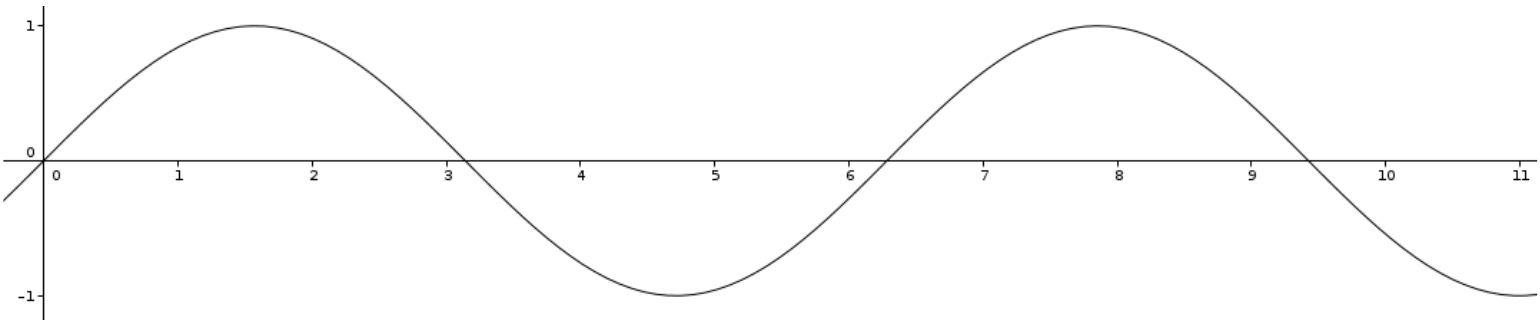
\includegraphics[width=.9\linewidth]{./img/transversalboelge.png}
\end{center}
\end{minipage}

\section*{Interferens}
\label{sec:orgd0c56b8}
\begin{minipage}{0.3\linewidth}
\begin{itemize}
\item Hvad er interferens?

\item Brug figuren.
\end{itemize}
\end{minipage}
\vline
\begin{minipage}{0.68\linewidth}
\begin{center}
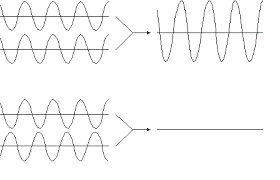
\includegraphics[width=.9\linewidth]{./img/Interferens.png}
\end{center}
\end{minipage}

\vfill

\section*{Bølgetyper}
\label{sec:org62c45b9}

\begin{minipage}{0.3\linewidth}
\begin{itemize}
\item Hvilke bølgetyper er der?

\item Eksempler fra naturen?
\end{itemize}
\end{minipage}
\vline
\begin{minipage}{0.7\linewidth}
\end{minipage}


\vfill

\section*{Det elektromagnetiske spektrum}
\label{sec:orgfdc5fe5}

\begin{minipage}{0.3\linewidth}
\begin{itemize}
\item I hvilket bølgelængdeinterval ligger synligt lys i EM-spektret?

\item Hvilke bølgerlængder hører til de farver, vi mennesker kan se?
\end{itemize}
\end{minipage}
\vline
\begin{minipage}{0.7\linewidth}
\end{minipage}
\end{document}
